\section{Method}

\begin{figure*}[t]\centering
\documentclass[tikz,border=10pt]{standalone}
\usepackage{amsmath,amssymb}
\usepackage{xcolor}
\usepackage{tikz}
\usetikzlibrary{positioning,calc,arrows.meta}

% ---------------- palette (colorblind-friendly) ----------------
\definecolor{netblue}{RGB}{31,119,180}
\definecolor{uncorange}{RGB}{216,100,20}
\definecolor{calteal}{RGB}{22,155,122}
\definecolor{fwd}{RGB}{65,65,65}

\tikzset{
  block/.style={draw=gray!65,fill=gray!7,rounded corners=2.5pt,align=center,inner sep=4pt,line width=0.7pt},
  oblock/.style={draw=netblue!85,fill=netblue!6,rounded corners=2.5pt,align=center,inner sep=4pt,line width=0.95pt},
  ublock/.style={draw=uncorange!90,fill=uncorange!6,rounded corners=2.5pt,align=center,inner sep=4pt,line width=0.95pt},
  lossnode/.style={circle,draw=gray!65,fill=white,minimum size=7.4mm,inner sep=0pt,line width=0.7pt,font=\footnotesize},
  sgnode/.style={circle,draw=gray!60,fill=gray!20,minimum size=7mm,inner sep=0pt,font=\footnotesize\bfseries,line width=0.7pt},
  sgbadge/.style={rectangle,rounded corners=1.5pt,draw=gray!55,fill=gray!18,inner sep=2.2pt,font=\tiny\bfseries,line width=0.5pt,text=black},
  smallhead/.style={draw=gray!65,fill=gray!8,rounded corners=1.5pt,minimum width=9.5mm,minimum height=5.6mm,inner sep=0pt,font=\footnotesize,line width=0.7pt},
  flow/.style={-{Latex[length=2.1mm,width=1.9mm]},line width=0.85pt,fwd},
  gradw/.style={-{Latex[length=2.8mm,width=2.5mm]},line width=1.3pt,netblue},
  gradth/.style={-{Latex[length=2.8mm,width=2.5mm]},line width=1.3pt,uncorange},
  dashcal/.style={-{Latex[length=2mm,width=1.8mm]},dashed,line width=0.9pt,calteal},
}

\begin{document}
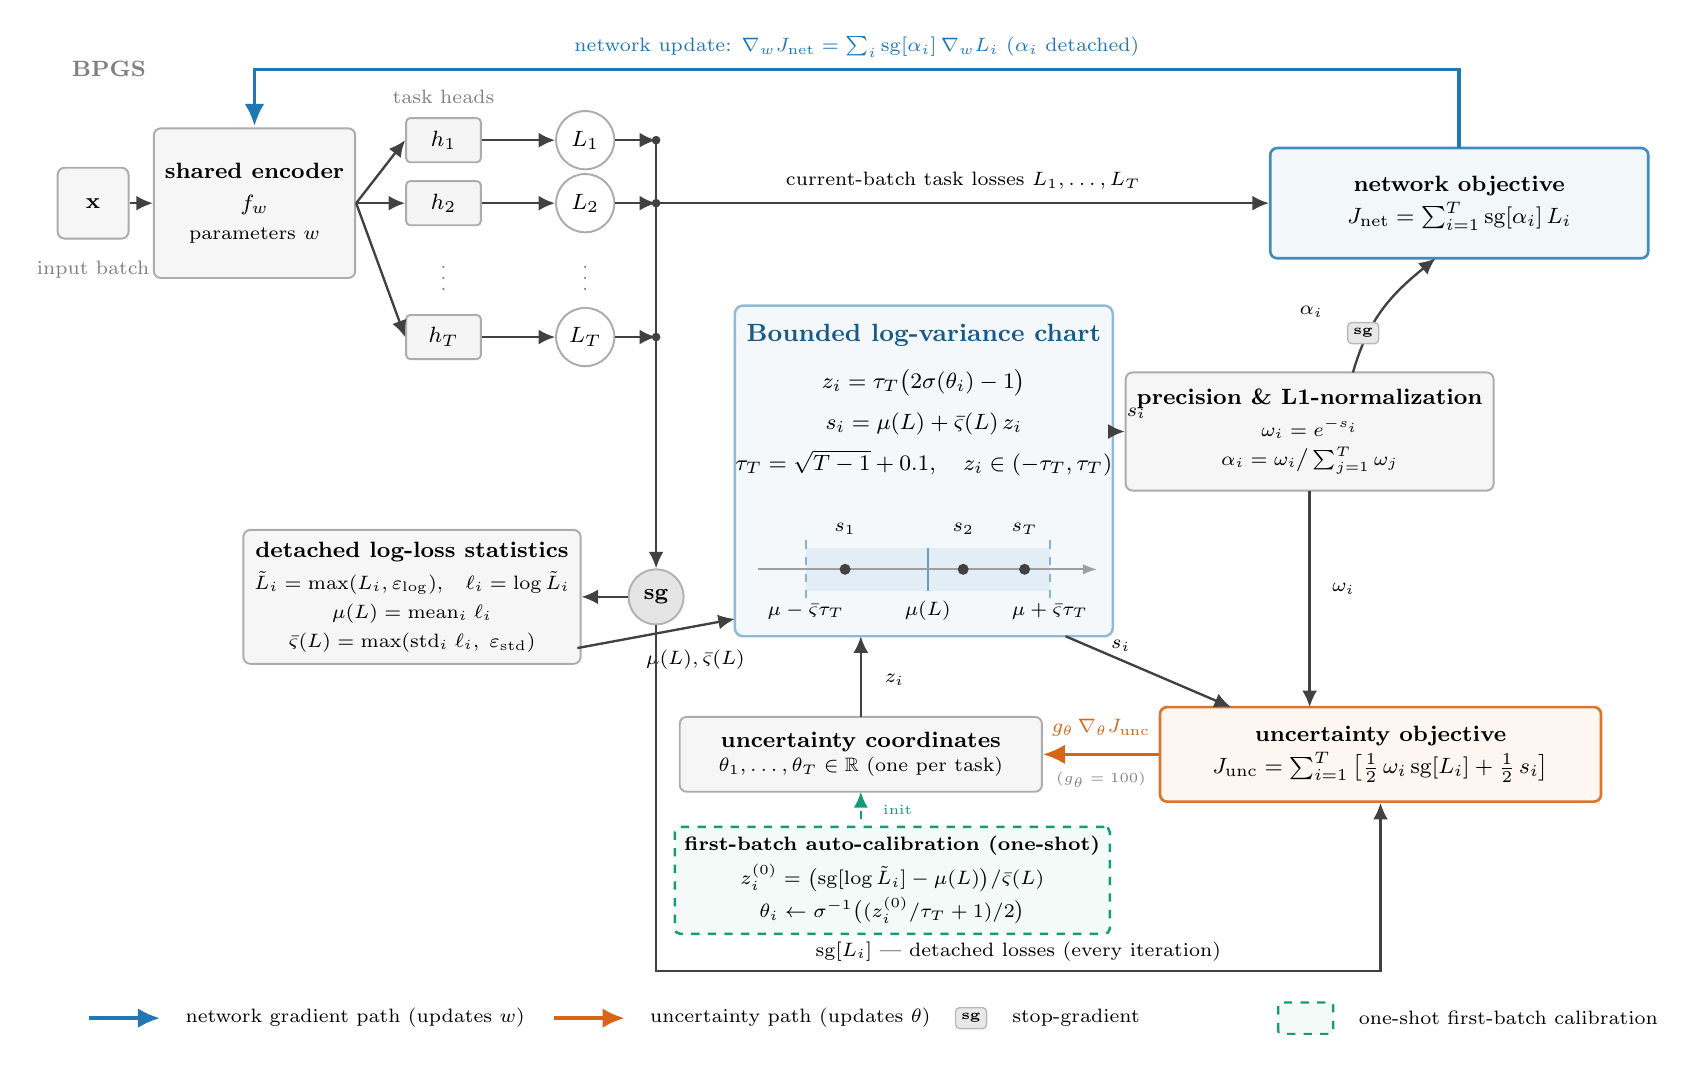
\begin{tikzpicture}[font=\footnotesize]

% ================= bounded chart panel (background) =================
\filldraw[fill=netblue!5,draw=netblue!50,rounded corners=3pt,line width=0.9pt]
  (8.7,2.5) rectangle (13.5,6.7);

% ================= forward pass =================
\node[block,minimum width=9mm,minimum height=9mm] (input) at (0.55,8.0) {$\mathbf{x}$};
\node[font=\scriptsize,gray] at (0.55,7.15) {input batch};

\node[block,minimum width=19mm,minimum height=19mm] (enc) at (2.6,8.0)
  {\textbf{shared encoder}\\[2pt] $f_{w}$\\[1pt] {\scriptsize parameters $w$}};

\node[smallhead] (h1) at (5.0,8.8) {$h_1$};
\node[smallhead] (h2) at (5.0,8.0) {$h_2$};
\node[font=\scriptsize,gray] at (5.0,7.15) {$\vdots$};
\node[smallhead] (hT) at (5.0,6.3) {$h_T$};
\node[font=\scriptsize,gray] at (5.0,9.35) {task heads};

\node[lossnode] (L1) at (6.8,8.8) {$L_1$};
\node[lossnode] (L2) at (6.8,8.0) {$L_2$};
\node[font=\scriptsize,gray] at (6.8,7.15) {$\vdots$};
\node[lossnode] (LT) at (6.8,6.3) {$L_T$};

\draw[flow] (input.east) -- (enc.west);
\draw[flow] (enc.east) -- (h1.west);
\draw[flow] (enc.east) -- (h2.west);
\draw[flow] (enc.east) -- (hT.west);
\draw[flow] (h1.east) -- (L1.west);
\draw[flow] (h2.east) -- (L2.west);
\draw[flow] (hT.east) -- (LT.west);

% ---- loss bus ----
\draw[flow] (L1.east) -- (7.7,8.8);
\draw[flow] (L2.east) -- (7.7,8.0);
\draw[flow] (LT.east) -- (7.7,6.3);

% ================= stop-gradient node + statistics =================
\node[sgnode] (sgn) at (7.7,3.0) {sg};

\node[block,minimum width=42mm,minimum height=17mm] (stats) at (4.6,3.0)
  {\textbf{detached log-loss statistics}\\[2pt]
   {\scriptsize $\tilde L_i=\max(L_i,\varepsilon_{\log})$,~~ $\ell_i=\log\tilde L_i$}\\[1pt]
   {\scriptsize $\mu(L)=\mathrm{mean}_i\;\ell_i$}\\[1pt]
   {\scriptsize $\bar\varsigma(L)=\max(\mathrm{std}_i\;\ell_i,\;\varepsilon_{\mathrm{std}})$}};

\draw[flow] (sgn.west) -- (stats.east);
\draw[flow] (6.7,2.35) -- (8.7,2.72);
\node[font=\scriptsize] at (8.2,2.2) {$\mu(L),\bar\varsigma(L)$};

% ================= chart internals =================
\node[font=\small\bfseries,text=netblue!75!black] at (11.1,6.32) {Bounded log-variance chart};
\node at (11.1,5.72) {$z_i=\tau_T\big(2\sigma(\theta_i)-1\big)$};
\node at (11.1,5.20) {$s_i=\mu(L)+\bar\varsigma(L)\,z_i$};
\node at (11.1,4.70) {$\tau_T=\sqrt{T-1}+0.1,\quad z_i\in(-\tau_T,\tau_T)$};

\fill[netblue!13] (9.6,3.08) rectangle (12.7,3.62);
\draw[dashed,netblue!55,line width=0.6pt] (9.6,2.98)  -- (9.6,3.72);
\draw[dashed,netblue!55,line width=0.6pt] (12.7,2.98) -- (12.7,3.72);
\draw[netblue!70,line width=0.8pt] (11.15,3.08) -- (11.15,3.62);
\draw[-{Latex[length=1.8mm]},gray!75,line width=0.7pt] (9.0,3.35) -- (13.3,3.35);

\node[font=\scriptsize] at (9.6,2.82)  {$\mu-\bar\varsigma\tau_T$};
\node[font=\scriptsize] at (11.15,2.82) {$\mu(L)$};
\node[font=\scriptsize] at (12.7,2.82) {$\mu+\bar\varsigma\tau_T$};

\fill[fwd] (10.1,3.35)  circle (0.07);
\fill[fwd] (11.6,3.35)  circle (0.07);
\fill[fwd] (12.38,3.35) circle (0.07);
\node[font=\scriptsize] at (10.1,3.86)  {$s_1$};
\node[font=\scriptsize] at (11.6,3.86)  {$s_2$};
\node[font=\scriptsize] at (12.38,3.86) {$s_T$};

% ================= uncertainty coordinates + calibration =================
\node[block,minimum width=46mm,minimum height=9.5mm] (theta) at (10.3,1.0)
  {\textbf{uncertainty coordinates}\\[-1pt]
   {\scriptsize $\theta_1,\dots,\theta_T\in\mathbb{R}$ (one per task)}};

\draw[flow] (10.3,1.475) -- (10.3,2.5);
\node[font=\scriptsize,anchor=west] at (10.48,1.95) {$z_i$};

\node[draw=calteal,dashed,fill=calteal!5,rounded corners=2pt,line width=0.9pt,
      align=center,inner sep=3.5pt,font=\scriptsize] (calib) at (10.7,-0.6)
  {\textbf{first-batch auto-calibration (one-shot)}\\[2pt]
   $z_i^{(0)}=\big(\mathrm{sg}[\log\tilde L_i]-\mu(L)\big)/\bar\varsigma(L)$\\[1pt]
   $\theta_i\leftarrow\sigma^{-1}\big((z_i^{(0)}/\tau_T+1)/2\big)$};

\draw[dashcal] (10.3,0.18) -- (10.3,0.525);
\node[font=\tiny,text=calteal,anchor=west] at (10.46,0.3) {init};

% ================= precision & normalization =================
\node[block,minimum width=40mm,minimum height=15mm] (prec) at (16.0,5.1)
  {\textbf{precision \& L1-normalization}\\[2pt]
   {\scriptsize $\omega_i=e^{-s_i}$}\\[1pt]
   {\scriptsize $\alpha_i=\omega_i\big/\sum_{j=1}^{T}\omega_j$}};

\draw[flow] (13.5,5.1) -- (prec.west);
\node[font=\scriptsize] at (13.8,5.33) {$s_i$};

% ================= split objectives =================
\node[oblock,minimum width=48mm,minimum height=14mm] (Jnet) at (17.9,8.0)
  {\textbf{network objective}\\[2pt]
   {\footnotesize $J_{\mathrm{net}}=\sum_{i=1}^{T}\mathrm{sg}[\alpha_i]\,L_i$}};

\node[ublock,minimum width=56mm,minimum height=12mm] (Junc) at (16.9,1.0)
  {\textbf{uncertainty objective}\\[2pt]
   {\footnotesize $J_{\mathrm{unc}}=\sum_{i=1}^{T}\big[\tfrac{1}{2}\,\omega_i\,\mathrm{sg}[L_i]+\tfrac{1}{2}\,s_i\big]$}};

% bus -> J_net (raw losses, not detached)
\draw[flow] (7.7,8.0) -- (Jnet.west);
\node[font=\scriptsize] at (11.6,8.28) {current-batch task losses $L_1,\dots,L_T$};

% alpha -> J_net with stop-gradient badge
\draw[flow] (16.55,5.85) .. controls (16.75,6.55) and (17.05,6.85) .. (17.6,7.3);
\node[sgbadge] at (16.68,6.35) {sg};
\node[font=\scriptsize] at (16.02,6.62) {$\alpha_i$};

% chart outputs into J_unc
\draw[flow] (12.9,2.5) -- (15.0,1.6);
\node[font=\scriptsize] at (13.6,2.38) {$s_i$};
\draw[flow] (16.0,4.35) -- (16.0,1.6);
\node[font=\scriptsize,anchor=west] at (16.16,3.1) {$\omega_i$};

% detached losses into J_unc
\draw[flow] (sgn.south) -- (7.7,-1.75) -| (Junc.south);
\node[font=\scriptsize] at (12.3,-1.5) {$\mathrm{sg}[L_i]$ — detached losses (every iteration)};

% ================= gradient updates =================
\draw[gradth] (Junc.west) -- (theta.east);
\node[font=\scriptsize,text=uncorange] at (13.35,1.34) {$g_\theta\,\nabla_\theta J_{\mathrm{unc}}$};
\node[font=\tiny,gray] at (13.35,0.68) {$(g_\theta=100)$};

\draw[gradw] (17.9,8.7) -- (17.9,9.7) -- (2.6,9.7) -- (2.6,8.98);
\node[font=\scriptsize,text=netblue] at (10.25,9.98)
  {network update: $\nabla_w J_{\mathrm{net}}=\sum_i \mathrm{sg}[\alpha_i]\,\nabla_w L_i$  ($\alpha_i$ detached)};

\node[font=\footnotesize\bfseries,gray] at (0.75,9.7) {BPGS};

% ================= bus junctions (drawn last) =================
\fill[fwd] (7.7,8.8) circle (0.055);
\fill[fwd] (7.7,8.0) circle (0.055);
\fill[fwd] (7.7,6.3) circle (0.055);
\draw[flow] (7.7,8.8) -- (sgn.north);

% ================= legend =================
\draw[gradw] (0.5,-2.35) -- (1.4,-2.35);
\node[font=\scriptsize,anchor=west] at (1.6,-2.35) {network gradient path (updates $w$)};
\draw[gradth] (6.4,-2.35) -- (7.3,-2.35);
\node[font=\scriptsize,anchor=west] at (7.5,-2.35) {uncertainty path (updates $\theta$)};
\node[sgbadge] at (11.7,-2.35) {sg};
\node[font=\scriptsize,anchor=west] at (12.1,-2.35) {stop-gradient};
\draw[draw=calteal,dashed,fill=calteal!5,rounded corners=1pt,line width=0.8pt]
  (15.6,-2.55) rectangle (16.3,-2.15);
\node[font=\scriptsize,anchor=west] at (16.5,-2.35) {one-shot first-batch calibration};

\end{tikzpicture}
\end{document}
\caption{Schematic overview of BPGS. For each batch, the shared encoder $f_w$ produces $T$ task
losses $L_1,\dots,L_T$. A stop-gradient branch computes log-loss statistics $\mu(L)$ and
$\bar\varsigma(L)$, which anchor a batch-conditional bounded chart: each learnable coordinate
$\theta_i$ is squashed to $z_i=\tau_T(2\sigma(\theta_i)-1)\in(-\tau_T,\tau_T)$ with
$\tau_T=\sqrt{T-1}+0.1$ and mapped affinely to
$s_i=\mu(L)+\bar\varsigma(L)z_i\in(\mu-\bar\varsigma\tau_T,\,\mu+\bar\varsigma\tau_T)$.
Precisions $\omega_i=e^{-s_i}$ are L1-normalized into weights $\alpha_i$. Optimization is split:
the network pass minimizes $J_{\mathrm{net}}=\sum_i\mathrm{sg}[\alpha_i]L_i$ w.r.t.\ $w$ with
detached weights, while the uncertainty pass minimizes
$J_{\mathrm{unc}}=\sum_i[\tfrac12\omega_i\mathrm{sg}[L_i]+\tfrac12 s_i]$ w.r.t.\ $\theta$ using
detached losses and statistics with gradient scale $g_\theta=100$. A one-shot inverse-sigmoid
auto-calibration initializes $\theta$ from the first batch; both passes use current-batch losses
at every iteration.}
\label{fig:bpgs_overview}
\end{figure*}

\subsection{Problem setup}
Let $T$ denote the number of tasks, let $w$ denote the shared network parameters, and let
\begin{equation}
L(w) = \bigl(L_1(w), \dots, L_T(w)\bigr)
\end{equation}
collect the raw task losses for the current batch. The goal is to construct adaptive task weights that remain informative when the task losses differ substantially in scale. BPGS does this by learning one latent uncertainty coordinate per task and mapping that coordinate into a bounded log-variance chart.

\subsection{Canonical BPGS chart}
For the canonical batch-aware variant, BPGS computes detached log-loss statistics
\begin{equation}
\widetilde L_i = \max(L_i, \varepsilon_{\log}), \qquad
\mu(L) = \frac{1}{T}\sum_{i=1}^{T}\operatorname{sg}[\log \widetilde L_i],
\end{equation}
and
\begin{equation}
\bar{\varsigma}(L) =
\max\!\left(
\sqrt{\frac{1}{T}\sum_{i=1}^{T}\bigl(\operatorname{sg}[\log \widetilde L_i] - \mu(L)\bigr)^2},
\varepsilon_{\mathrm{std}}
\right).
\end{equation}
Each task has a learnable uncertainty coordinate $\theta_i \in \mathbb{R}$. Using the task-count-dependent latent radius
\begin{equation}
\tau_T = \sqrt{T-1}+0.1,
\label{eq:tau}
\end{equation}
we define the bounded latent coordinate
\begin{equation}
z_i(\theta_i) = \tau_T \bigl(2\sigma(\theta_i)-1\bigr),
\end{equation}
where $\sigma(\cdot)$ is the logistic sigmoid. The canonical BPGS log-variance is then
\begin{equation}
s_i(\theta_i;L) = \mu(L) + \bar{\varsigma}(L)\, z_i(\theta_i).
\end{equation}

The radius in Eq.~\eqref{eq:tau} follows from the geometry of a population-standardized
$T$-vector. When the safeguards are inactive, its coordinates have zero mean and unit average
square. If one coordinate has magnitude $M$, the other $T-1$ coordinates must sum to $-M$;
their squared sum is minimized when they are equal. Hence
$T \ge M^2+(T-1)(M/(T-1))^2$, giving $M\le\sqrt{T-1}$. The added $0.1$ is a numerical margin
that keeps first-batch inverse-sigmoid calibration away from the chart boundary.
The corresponding task precision is
\begin{equation}
\omega_i(\theta_i;L) = e^{-s_i(\theta_i;L)},
\end{equation}
and the network weight is its L1-normalized version
\begin{equation}
\alpha_i(\theta_i;L) =
\frac{\omega_i(\theta_i;L)}{\sum_{j=1}^{T}\omega_j(\theta_j;L)}.
\end{equation}

This chart expresses each task relative to the current batch while keeping the learnable coordinate
inside a finite range.

In the canonical configuration, BPGS performs a one-shot auto-calibration on the first observed batch,
mapping its detached log-loss statistics into the bounded chart before the first network update. The
ablations test this initialization separately from the batch-aware chart.

\subsection{Split optimization objectives}
BPGS uses separate objectives for the network parameters and the uncertainty coordinates. The network objective is
\begin{equation}
J_{\mathrm{net}}(w \mid \theta, L)
=
\sum_{i=1}^{T} \operatorname{sg}\!\left[\alpha_i(\theta_i;L)\right] L_i,
\end{equation}
where $\operatorname{sg}[\cdot]$ denotes stop-gradient. The uncertainty objective is
\begin{equation}
J_{\mathrm{unc}}(\theta \mid L)
=
\sum_{i=1}^{T}
\left[
\frac{1}{2}\omega_i(\theta_i;L)\operatorname{sg}[L_i]
+
\frac{1}{2}s_i(\theta_i;L)
\right].
\label{eq:unc}
\end{equation}
Equation~\eqref{eq:unc} has the same algebraic form as the scalar uncertainty objective of
classical homoscedastic uncertainty weighting \cite{kendall2018}, but it is not the same
optimization problem. Kendall's log-variance is unconstrained, whereas BPGS confines $s_i$ to a
batch-conditional interval; their fixed-point structures therefore differ even though the
objective forms coincide.

The implemented uncertainty update uses a fixed gradient scale $g_\theta=100$. This constant is
used across the reported BPGS configurations to compensate for the smaller uncertainty-gradient
magnitudes; it changes the update speed, not the weighting rule. Appendix~\ref{app:reproducibility}
lists this and the remaining optimizer settings.

At each iteration, both passes use the current-batch losses. The network update uses detached
normalized weights in $J_{\mathrm{net}}$, while the separate uncertainty update uses $J_{\mathrm{unc}}$
with detached losses and batch statistics; this keeps weight adaptation from reshaping the network
gradient in the same update.

\subsection{Batch-conditional boundedness}
\label{sec:boundedness}
The key formal property used in our robustness framing is conditional boundedness with respect to the current batch. For any fixed batch $L$ and any finite $\theta_i$,
\begin{equation}
\mu(L)-\bar{\varsigma}(L)\tau_T
<
s_i(\theta_i;L)
<
\mu(L)+\bar{\varsigma}(L)\tau_T.
\end{equation}
This follows immediately from $\sigma(\theta_i)\in(0,1)$, which implies
\begin{equation}
z_i(\theta_i)\in(-\tau_T,\tau_T).
\end{equation}
Substituting this interval into the affine map defining $s_i$ gives the stated bound. Consequently, for any fixed batch, the induced precision $\omega_i(\theta_i;L)$ is strictly positive and remains inside a finite interval. The claim is therefore batch-conditional rather than globally independent of the observed loss statistics.

Boundedness alone does not ensure learnability near the boundary: as $z_i$ approaches
$\pm\tau_T$, the sigmoid derivative vanishes and recovery can become difficult. We therefore
examined the logged main-paper trajectories (Appendix~\ref{app:chart_behavior}). The largest
observed ratio was $|z_i|/\tau_T=0.93$ (NYUv2, initialization); the final-epoch caps were at most
0.84 on NYUv2, 0.69 on Yeast, and 0.89 on RF1. The closest observed point retained a derivative
factor of about $0.033$ (13\% of its maximum), and the final epochs reached about $0.074$.
Thus no logged run exhibited boundary locking, although this empirical margin is not a guarantee.

\subsection{Uniform rescaling invariance}
\label{sec:invariance}
\begin{proposition}[Uniform rescaling invariance]
\label{prop:invariance}
Let $L'_i=cL_i$ for every task and some $c>0$. If the numerical safeguards
$\varepsilon_{\log}$ and $\varepsilon_{\mathrm{std}}$ are inactive on both batches, then
$\alpha_i(\theta_i;L')=\alpha_i(\theta_i;L)$ for all $i$. First-batch auto-calibration also
produces the same initial $\theta_i$ values under the same rescaling.
\end{proposition}

\begin{proof}
Uniform rescaling adds $\log c$ to every log-loss. Therefore $\mu(L')=\mu(L)+\log c$ while
$\bar{\varsigma}(L')=\bar{\varsigma}(L)$, and $z_i(\theta_i)$ is unchanged. Hence
$s_i(\theta_i;L')=s_i(\theta_i;L)+\log c$, so each raw precision is multiplied by the same
factor $1/c$, which cancels in the L1 normalization. The standardized coordinates used for
first-batch calibration are unchanged by the same additive shift.
\end{proof}

The proposition concerns normalized weights on a fixed batch, not an entire optimizer trajectory or
final predictive metrics; the pure-rescaling experiment tests that broader empirical behavior.
